\section{Методы сравнения моделей}

\subsection{Моделирование канала с постоянной битовой
скоростью и получение характеристик качества
обслуживания}

\subsubsection{Общий принцип использования характеристик
качества обслуживания для сравнения моделей.}

\hspace{3pt}
Помимо статистических методов сравнения моделей используется
\cite{}
и совершенно иной подход: сравнение характеристик качества
обслуживания (Quality of Service, QoS) для простейшего
канала передачи данных.

Центральная идея данного подхода заключается в следующем:
предполагается, что наиболее подходящая модель будет демонстрировать
схожие с оригинальным видео показатели качества обслуживания
для любого канала передачи данных. Моделируется канал с постоянной
битовой скоростью (Constant Bit-Rate, CBR) в качестве входных
данных для которого служат пакеты, размеры которых соответствуют
размерам кадров в оригинальном видео и в реализации,
сгенерированной моделями. Для каждой модели производится сравнение
параметров качества обслуживания с параметрами, полученными
для исходного видео. Наиболее подходящей признаётся та модель,
которая в наименьшей степени отклоняется от показателей оригинального
видео.

Данный подход оправдан по следующим причинам: во-первых,
он позволяет оценивать модели по тем критериям, которые
будут играть прямую роль при дальнейшем использовании модели.
Предполагается, что модель должна облегчить задачу проектирования
сети передачи данных. Следовательно, лучшей должна быть признана
та модель, которая будет демонстрировать наиболее близкое
к оригиналу поведение при передаче по каналу связи.

Во-вторых, на критерии качества обслуживания в первую очередь
влияет характер следования размеров сжатых кадров друг за
другом, а не только статическое распределение размеров
кадров \cite{}.
Эти критерии позволяют подробнее исследовать поведение сжатой
видеопоследовательности во времени. Информация такого
рода отсутствует в результатах исследования стационарного
распределения. Исследование автокорреляционной функции
также не даст достаточной информации о ``скученности'' размеров
кадров во времени.

\subsubsection{Модель канала передачи данных при
сравнительном анализе моделей выхода видеокодера}
\hspace{3pt}

Сравнительный анализ моделей передачи видеотрафика посредством
получения характеристик качества обслуживания требует формализации
модели канала передачи данных. В рамках данной работы
рассматривается канал с постоянной битовой скоростью (англ.
Constant Bit-Rate, CBR) с буфером на входе. Схематически
используемая модель изображена на Рис.~\ref{fig:delay_jitter_model}.

\begin{figure}[h]
    \begin{center}
        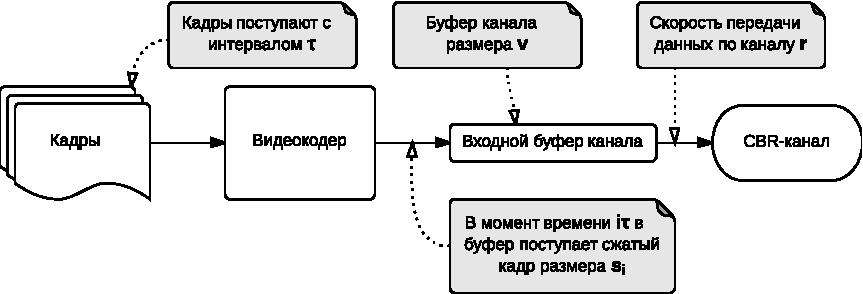
\includegraphics[width=\textwidth]{delay_jitter_model.pdf}
    \end{center}
    \caption{Модель системы передачи видеотрафика для исследования
    характеристик качества обслуживания}
    \label{fig:delay_jitter_model}
\end{figure}

Процесс передачи данных в расматриваемой модели происходит следующим
образом: с интервалом $\tau$ в момент $\tau i$ с выхода
кодера в буфер канала объёмом $v$, в котором на данный момент
находится $k_i$ байт, поступают $s_i$ байт информации, $i = 1 \dots N$.
Если происходит переполнение буфера, излишек считается утерянным.
Содержимое буфера передаётся по каналу с фиксированной скоростью
$v$. Если буфер оказывается пустым, канал ожидает поступления
новых данных, после чего возобновляет передачу.
Эта модель значительно проще реальных систем передачи данных
и исходит из следующих допущений:

\begin{itemize}
    \item видеокодер способен обеспечивать стабильный период следования кадров $\tau = const$;
    \item используется канал с постоянной битовой скоростью;
    \item не учитываются добавочные нагрузки на передачу заголовков пакетов
        и прочей служебной информации;
    \item не рассматривается буферизация на стороне получателя и вопросы начальной буферизации;
    \item не предпринимается попыток восстановления данных при переполнении
        буфера отправителя.
\end{itemize}

Приведённые допущения оправданы в силу того, что полноценное моделирование
канала передачи информации не приведёт к более достоверному сравнению
моделей видеотрафика, значительно усложнив при этом задачу моделирования канала.


\subsubsection{Коэффициент потерь при переполнении буфера}
\hspace{3pt}

Исследование коэффициента потери при предачи по каналу
с фиксироованным буфером на входе (``тест с текущим ведром'',
англ. Leaky-Bucket Test) является основным
методом исследования неравномерности трафика (burstiness),
применявшимся с первых исследований передачи VBR-трафика
\cite{}.
Коэффициент потери ячеек (англ. Cell Loss Rate) являлся
важнейшей характеристикой качества обслуживания при передаче
данных по сети ATM.

Пусть есть канал с фиксированной постоянной пропускной
способностью $r$, на входе которого стоит буфер размера $v$.
На вход канала с постоянной частотой поступают сжатые
кадры. Далее приведено пошаговое описание теста, осуществляемого
при помощи имитационного моделирования описанного канала.

За шаг времени $\tau$ примем интервал между поступлениями
кадров. Пусть на момент поступления очередного кадра размера
$s_i$ в буфере осталось $k \in [0; v]$ непереданных байт.
В случае, если текущий не может быть сохранён
в буфере ($ns_i = s_i + k > v$), буфер переполняется и излишек $o_i = ns_i - v$
считается потерянным. К появлению следующего кадра
в буфере останется $k \leftarrow \max(\min(ns, v) - r\tau, 0)$ байт,
после чего процедура повторяется для следующего кадра.
Контроль целостности кадров в данном тесте не осуществляется.

Метрикой каждой последовательности размеров кадров будем считать
долю потерянных байтов к общему объёму передаваемых данных
в последовательности:

\begin{equation}
    \eta = \frac{\sum_i o_i}{\sum_i s_i},
\end{equation}
суммирование ведётся по входящей последовательности кадров.

Расмотренная модель канала параметризуется двумя параметрами:
размером буфера $v$ и пропускной способностью на кадр $r\tau$.
Для получения релевантных результатов теста необходимо правильно
подбирать эти параметры в зависимости от статистических параметров
входной последовательности. Для определения области допустимых значений
необходимо рассмотреть данный канал как систему массового обслуживания
\cite{}
(СМО). В соответствии с расширенной нотацией Кендалла
\cite{},
данная модель имеет тип D/G/1/$v$, то есть распределение
вероятностей поступления заявок в систему детерминировано
(заявки поступают с интервалом $\tau^{-1}$), распределение
времени обслуживания произвольно и зависит от распределения
размеров кадров, очередь обслуживает один обработчик,
а объём очереди равен $v$. Существенно, что размер очереди
определяется не количеством слотов, а объёмом невыполненной
работы в очереди, в полным соответствии с аналогией ``текущего
ведра''.

Рассмотрение приведённой модели канала в качестве СМО позволяет
сформулировать граничные условия применимости данной модели
канала при сравнении различных моделей видеопоследовательностей:
в соответствии с условием стационарности СМО, интенсивность
входного потока заявок не должна превышать интенсивность обслуживания
\cite{},
следовательно

\begin{equation}
    \frac{\lambda}{\mu} = \frac{\overline{s}}{r\tau} \ < 1,
\end{equation}
интенсивность входного потока равна $\overline{s}/\tau$ байт/сек
(предполагается стационарность входного потока),
интенсивность обслуживания равна $r$ байт/сек по определению.
Таким образом, для обеспечения стационарного режима работы необходимо
установить пропускную способность канала большей, чем средний размер
кадра. Для установленной пропускной способности канала и для различных
последовательностей размеров кадров варьируется размер буфера в некотором
диапазоне от среднего размера кадров, полученные зависимости
сравниваются между собой.

\subsubsection{Задержка в получении кадра и джиттер}
\hspace{3pt}

В настоящее время мультимедиа данные, в том числе и трафик видеоконференций,
передаются преимущественно по IP-сетям, важнейшими критериями качества обслуживания
для которых
являются задержка в получении пакета (англ. delay) и джиттер, или дрожание
(англ. jitter), то есть отклонение в интервале поступления пакетов.

В целях сравнительного анализа моделей видеотрафика на основе задержки
и джиттера предлагается рассматривать модель канала, схожую с рассмотренной
при анализе коэффициента потерь, но с неограниченным буфером на входе.

В рамках данного теста передача осуществляется без потерь. В момент времени
$\tau i$ кадр под номером $i$ приходит в систему и заполняет $s_i$
байт в буфере. Канал передаёт содержимое буфера с постоянной скоростью
$r$ и в некоторый момент времени $t_i$ закончит передавать последний
байт кадра $i$. Промежуток времени между поступлением кадра в систему и полной
передачей кадра в канал $d_i = t_i - \tau i$ называется задержкой
и может рассматриваться как случайная величина, зависящая от
входного потока кадров и от пропускной способности канала $r$.

Джиттер характеризует степень неустойчивости интервалов появления
кадров на принимающей стороне канала. В некоторых источниках
\cite{}
джиттером называют дисперсию задержки, в других
\cite{}
--- производную задержки по времени. В работе используется
второе определение, так как оценка джиттера таким способом
используется на приёмной стороне, для которой данные о поступлении
кадров в систему недоступны.

Совокупность промежутков между получением двух соседних кадров $t_{i+1} - t_i$
называется джиттером и может быть получена на основе задержки следующим образом:

\begin{equation}
    \left\{
    \begin{aligned}
        d_i &= t_i - \tau i\\
        d_{i+1} &= t_{i+1} - \tau (i+1),\\
    \end{aligned}
    \right.
\end{equation}
\begin{equation}
    \begin{aligned}
    d_{i+1} - d_i &= t_{i+1} - \tau i - \tau - t_i + \tau i\\
                  &= t_{i+1} - t_i - \tau\\
    \Longrightarrow t_{i+1} - t_i &= d_{i+1} - d_i + \tau
    \end{aligned}
\end{equation}

Рассуждения, аналогичные приведённым при рассмотрении коэффициента
потерь для определения граничной пропускной способности канала,
применимы и при оценке задержки и джиттера.

Моделирование канала для получения значений задержек было
осуществлено при помощи двух методик имитационного моделирования:
дискретно-событийного моделирования и аналитического метода.
Далее приведено описание обеих методик.

В рамках дискретно-событийного моделирования временная шкала
разбивается на кванты времени длительностью $q$. В качестве 
параметров модели указывается количество квантов времени в
периоде следования кадров и количество байт, передаваемых
каналом за квант времени $b$. Непереданный остаток от текущего
кадра и его индекс хранятся в переменных. На каждом шаге
алгоритма происходит уменьшение остатка от текущего кадра
на $b$ байт. После того, как текущий кадр передан целиком
(остаток стал меньшим либо равным нулю), в качестве задержки
для текущего кадра сохраняется разность текущего времени со
временем поступления кадра $i \tau$ (может быть вычислено аналитически в любой момент).
Далее, в случае, если время появления следующего кадра в системе
ещё не наступило (буфер опустел), программа инкрементирует
счётчик времени до прихода следующего кадра. Если же следующий
кадр уже пребывает в системе, моделирующая программа принимает
этот кадр за текущий и повторяет описанную процедуру.

Данный подход имеет ряд преимуществ: с его помощью удаётся
избежать явного отслеживания состояния буфера,
он максимально точно отражает логику передачи данных в реальном
канале с буфером и потенциально данный подход можно
без особых изменений применить и для канала с переменной
битовой скоростью, как и для случая неравномерного поступления
кадров в буфер или для более сложных политик передачи данных
(очередь с приоритетами и пр.). Однако в рамках данного подхода приходится
учитывать пограничные случаи, такие как возможность при
непустом буфере в рамках одного кванта передавать
данные от нескольких кадров. Кроме того, данный подход вынуждает
использующего моделирующую программу в явном виде указывать
ненужные с точки зрения анализа моделей параметры, такие,
как количество квант на кадр.

Вышеизложенные соображения позволяют сделать вывод об
избыточности дискретно-событийного метода имитационного
моделирования в рамках задачи нахождения задержки
и джиттера в канале с постоянной пропускной способностью.
В связи с этим был предложен альтернативный метод
моделирования, в большей степени полагающийся на
заданные свойства системы (равномерное поступление
кадров на вход, CBR-канал) и потому более простой
в реализации.

За один такт модели примем поступление очередного
$i$-го кадра в систему. Пусть на этот момент в
буфере отправителя находится $b_i$ байт информации,
пропускная способность равна $r\tau$ байт на кадр.
Текущий кадр будет передан после того, как будет
передано содержимое буфера, поэтому время передачи
текущего кадра вычисляется следующим образом:

\begin{equation}
    d_i = \frac{s_i + b_i}{r\tau}.
\end{equation}

К моменту поступления следующего кадра в буфере
останется $b_{i+1} = \max(s_i + b_i - r\tau, 0)$
байт. Это значение принимается за текущее состояние
буфера и алгоритм переходит к следующему кадру.

Помимо простоты данного подхода следует отметить и
тот факт, что результирующая задержка не дискретизована
до размера кванта, поэтому данный метод демонстрирует
большую точность при большей производительности.
Результаты моделирования обоими способами совпадают
с точностью до размера кванта в дискретно-событийной модели.
В ходе сравнения различных моделей видеотрафика использовался
аналитический метод моделирования канала.

Полученные последовательности задержек $d_i$ и интервалов
между появлениями кадра на получателе $\Delta t_i$, $i = 1 \dots N$
рассматриваются как выборки случайной величины, для которой
могут быть получены стандартные статистические характеристики.
Именно математические ожидания задержки и джиттера выбраны
в данной работе в качестве характеристик
конкретной модели при фиксированных параметрах канала.
